\chapter{Overview}
\label{ch:overview}

The main contribution of this dissertation is {\em a suite of solutions to make 
data-driven QoE optimization practical} -- one can substantially improve QoE 
by maintaining a global view of up-to-date network conditions based on the 
QoE information collected from many endpoints.
Our solutions achieve this through novel algorithm designs and system 
implementation that integrate machine learning techniques with domain-specific
insights.
%We  demonstrate that one can achieve substantial QoE improvement
%by utilizing measurement data already available to today's application 
%providers and integrating domain-specific insights with machine learning 
%techniques to make better real-time adaptation for client-side applications.
%In this chapter, we give an overview of our solutions, the key insight
%behind our solutions, and a perspective of how this solution compared 
%to prior efforts of Internet quality optimization and applying data-driven
%in the networking literature.

This chapter is organized as follows.
We begin with an overview of the envisioned 
architecture of data-driven QoE optimization, 
called {\em Data-Driven Networking} or {\em \ddn} (Section~\ref{sec:overview:arch}).
%some illustrative examples of how different applications 
%may benefit from \ddn, and perspective of how this solution compared 
%to prior work.
Then we discuss the algorithmic and architectural challenges of \ddn in 
Section~\ref{sec:overview:challenges}, motivate the unifying insights behind
our solutions in Section~\ref{sec:overview:unifying}, and finally describe
the key ideas of our solutions in Section~\ref{sec:overview:solutions}.
%describes a suite of solutions inspired by the insight to address \ddn's
%challenges in the context of Internet video and Internet telephony.


\section{Formalizing \ddn}
\label{sec:overview:arch}

We begin a conceptual overview of the Data-Driven 
Networking (\ddn) paradigm (Section~\ref{subsec:overview:concept}),
and some illustrative examples of how different applications   
can benefit from \ddn (Section~\ref{subsec:overview:examples}).
We end this section by contrasting it to prior
approaches (Section~\ref{subsec:overview:contrast}).
%We end this section by identifying key factors that can impact 
%the potential benefits of \ddn.

\subsection{Conceptual Architecture}
\label{subsec:overview:concept}

\ddn is a new paradigm for designing the adaptation logic of 
end-to-end protocols (such as adaptive video streaming protocols). 
Unlike prior endpoint approaches, 
\ddn-based control loop is driven by real-time
{\em multi-session} (not single-session) view of 
{\em in-situ quality}~\cite{insitu} 
measurement (not active
measurements or indirect metrics), 
and {\em automatically tuned actuation algorithms} based
on data-driven insights (with little to no manual tuning).

A \ddn-enabled protocol has two additional components:
(a) the {\em client-side instrumentation} code which runs inside 
client-side application to measure client-perceived quality of 
each session and applies decisions made by \ddn; and 
(b) the {\em \ddn controller} which runs two loosely coupled steps:
\begin{enumerate}
\item Aggregate quality measurement from client-side 
instrumentation into a global view of up-to-date network conditions and 
some actionable insights.
\item Make control decisions based on the actionable insights, 
and send them to client-side instrumentation for execution.
\end{enumerate}

%Note that the \ddn paradigm is compatible to 
%the existing infrastructure operated by application 
%providers. For instance, many application providers 
%have already deployed client-side instrumentation to
%monitor client-side information in real-time and collect
%measurement for offline analytics (e.g.,~\cite{sigcomm11}).
%Many application providers also maintain a global control
%platforms (e.g.,~\cite{c3,via,footprint,chen2015end}) 
%where the \ddn controller can be implemented.

\ddn is aligned with several favorable technology trends, and can be 
readily deployed in the existing distribution infrastructures of Internet applications.
(1) Many application providers today have widely deployed client-side 
instrumentations that can collect real-time in-situ QoE data 
en masse from clients (e.g.,~\cite{sigcomm11,via,akamai-imc12,artizanetworks}). 
(2) Logically centralized control platforms are commonly deployed by many 
application providers (e.g., content providers~\cite{c3}, web services~\cite{footprint}) and CDN providers (e.g.,~\cite{chen2015end,mukerjee2015practical}).
(3) The emergence of large-scale data analytics platforms and cloud infrastructure 
provides the ability to extract insights efficiently from large corpses 
of data (e.g.,~\cite{spark}) and streams of updates 
(e.g.,~\cite{zaharia2013discretized}). 
%Such ability enables optimal decision making based on
%real-time data-driven predictions~\cite{velox-cidr}.


\begin{figure}[t!]
\centering
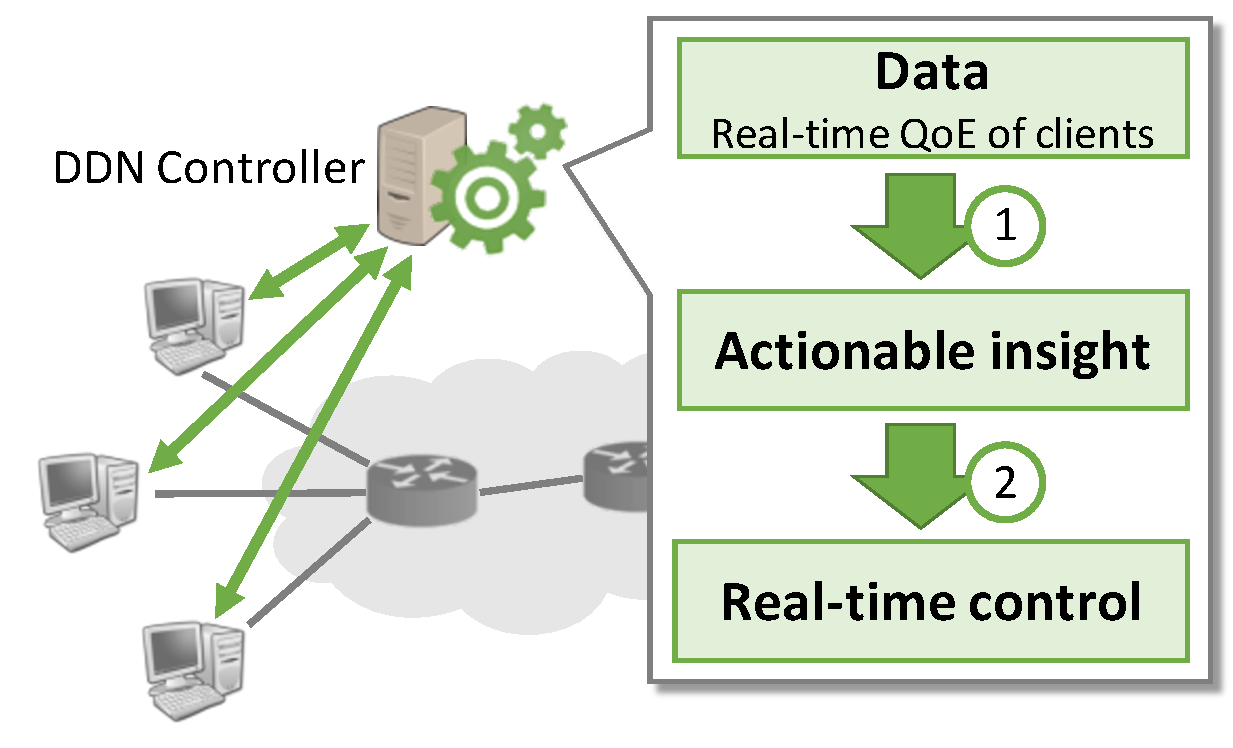
\includegraphics[width=0.6\textwidth]{figures/overview-ddn-arch.pdf}
%\vspace{-0.3cm}
\caption{Overview of the \ddn controller}
\label{fig:intro-contribution}
\end{figure}

\subsection{Contrast to Prior Work}
\label{subsec:overview:contrast}

\subsubsection{Compared to Prior Work on Quality Optimization}

We now put the \ddn approach to QoE optimization in perspective
using the taxonomy presented in Section~\ref{sec:related:quality}.
There are two classes of prior solutions: in-network solutions that change 
in-network devices, and endpoint solutions that rely on endpoint adaptations.

%In Section~\ref{sec:related:quality}, we have classified
%prior work on quality optimization along two dimensions:
%where in the network (in-network vs. endpoints), and
%which level in the protocol stack (application vs. lower layers).
%Using this taxonomy, \ddn should be classified as an 
%endpoint solution operating in the application layer.

\begin{itemize}

\item Unlike prior endpoint solutions which use only per-endpoint local 
information, decision making in \ddn is driven by information of multiple sessions. 
The core argument of \ddn is that {\em it is feasible to
maintain an accurate view of network conditions based on the QoE information
collected from many endpoints}.
%Traditional end-to-end adaptation protocols (e.g., TCP/DASH) 
%is driven by what is observed by a single session. In contrast, 
By extending the spatial scope of QoE measurement, 
\ddn can predict the quality of a session if it uses certain decision, 
as long as the decision has been used by 
some similar sessions.
\ddn is in part inspired by seminal work such as SPAND~\cite{spand},
and our contribution lies in providing end-to-end solutions to make \ddn
practical by leveraging the recent advances
in large-scale data analytics and domain-specific insights.
In short, \ddn retains the ethos of the endpoint approach, 
while addressing its lack of
visibility to network condition by leveraging an expended view 
across many endpoints.

\item Unlike in-network solutions or endpoint solutions operating 
in lower layers, \ddn enjoys the advantage that it has  
direct access to in-situ QoE measurement.
In \ddn, what to be ``sensed'' is exactly what to be optimized, 
i.e., quality perceived by all historical and ongoing sessions; 
not indirect signals on quality (e.g., acks 
or bandwidth), or active probes from a handful 
of vantage points (e.g., iPlane~\cite{iplaneosdi}). 
While in-situ quality data may compromise on the fidelity of 
individual measurement, they are far more efficient than 
alternatives in obtaining a panoramic and representative
 view of client-perceived quality from growingly diverse platforms~\cite{insitu}.
%and the lack of fidelity can be compensated by harnessing the ``unreasonable effectiveness of data''~\cite{google-data}.
Relying solely on in-situ quality data also serves pragmatic 
purposes as many application providers today already have 
a vested interest in measuring user-perceived quality for 
various reasons~\cite{sigcomm-qoe-workshop}.

\end{itemize}





%To understand the contrast between  \ddn and traditional 
%control planes, it is useful to revisit the two logical steps 
%in the workflow of {\em any} control plane 
%(Figure~\ref{fig:sensing-actuation}):
%{\em sensing}, which gives the feedback data to control plane, 
%and {\em actuation}, which turns the feedback data to control decisions.
%\ddn radically departs from non-\ddn designs on both fronts 
%with two definitive features.

%(Table~\ref{tab:ddn} provides some examples to contrast between \ddn and non-\ddn designs.)

%\begin{itemize}
%\item {\em Multi-session view:} 
%Sensing of \ddn is based on multiple sessions, rather than single session. 
%Traditional end-to-end adaptation protocols (e.g., TCP/DASH) 
%is driven by what is observed by a single session. In contrast, 
%By extending the spatial scope of sensing to many sessions, 
%\ddn can predict the quality of a decision even before a session 
%actually uses it, as long as the decision has been used by 
%some similar sessions.
%
%\item {\em In-situ quality:}
%In \ddn, what to be ``sensed'' is exactly what to be optimized, i.e., quality perceived by all historical and ongoing sessions; 
%not indirect signals on quality (e.g., acks~\cite{jacobson1988congestion} or bandwidth~\cite{bwe}), or active probes from a handful of vantage points (e.g., iPlane~\cite{iplaneosdi}). 
%While in-situ quality data may compromise on the fidelity of individual measurement, they are far more efficient than alternatives in obtaining a panoramic and representative view of client-perceived quality from growingly diverse platforms~\cite{insitu}.
%%and the lack of fidelity can be compensated by harnessing the ``unreasonable effectiveness of data''~\cite{google-data}.
%Relying solely on in-situ quality data also serves pragmatic purposes as many application providers today already have a vested interest in measuring user-perceived quality for various reasons~\cite{sigcomm-qoe-workshop,sigcomm12,krishnan2013video}.
%
%%\item {\bf Automatically tuned control logic:}
%%To take full advantage of the enriched sensing data, actuation algorithms of \ddn should be dynamically tuned by data-driven insights with little to no manual configuration.
%%Unlike today's protocols where handpicked constants are used as key parameters (e.g., init\_cwnd and initial video bitrate), \ddn picks parameters~\cite{remy} and control logic~\cite{cs2p} based on quality feedback which indicates what suit the current operating condition the best.
%%Meanwhile, the \ddn control logic also needs to handle the {\em downside} of having more data (e.g., lack of fidelity in client-side measurement, and whether the data source is trustworthy) by harnessing the ``unreasonable effectiveness of data''~\cite{google-data}.
%
%\end{itemize}


%\begin{table}[t!]
%\centering
%\resizebox{0.6\textwidth}{!}{%
%\begin{tabular}{@{}cccc@{}}
%\toprule
%\textbf{} & \multicolumn{2}{c}{\textbf{Sensing}} & \textbf{Actuation} \\ \midrule
%\textbf{} & \textit{Multi-session} & \textit{In-situ quality} & \textit{Auto-tuned} \\ \midrule
%%\rowcolor[HTML]{FFFE65} 
%DDN & \Checkmark & \Checkmark & \Checkmark \\
%TCP AIMD~\cite{jacobson1988congestion} & $\times$ & $\times$ & $\times$ \\
%PCC~\cite{pcc} & $\times$ & \Checkmark & \Checkmark \\
%OSPF, BwE~\cite{bwe} & \Checkmark & $\times$ & $\times$ \\
%iPlane~\cite{iplaneosdi} & \Checkmark & $\times$ & NA \\
%RemyCC~\cite{remy} & $\times$ & $\times$ & \Checkmark \\ \bottomrule
%\end{tabular}%
%}
%\vspace{0.3cm}
%\caption{Difference of \ddn to non-\ddn strategies.}
%\label{tab:ddn}
%\end{table}

%\subsection{Contrast to Prior Work on Data-Driven Optimization}
\subsubsection{Compared to Prior Work on Data-Driven Optimization}

In Section~\ref{sec:related:data}, we have described two types
of data-driven optimization in networked systems:
better parameter setting, and better run-time decision making.
Under this taxonomy, \ddn belongs to the second type, but with a 
key difference--in \ddn, decisions are driven by real-time data from 
many different
users or sessions, rather than a single user. 
This difference has two profound implications.
%, from the perspective of data-driven paradigm.
On one hand, the input data of \ddn is much larger both in scale 
and scope, allowing \ddn to learn a more accurately model
of the network conditions and make more informed decisions.
On the other hand, the input data of \ddn is collected from both
concurrent and history sessions with different client-side and
server-side characteristics, so the \ddn controller
cannot treat the data from different sessions identically when
using it to make decisions for a particular session; rather
it must take into account the potentially 
complex relationship between session-level 
features and QoE.


\subsection{Illustrative Examples}
\label{subsec:overview:examples}

Several early applications of \ddn from prior work have shown 
tremendous promise of this new paradigm.
%how \ddn can be adapted to various use cases 
%to exploit their potential benefits. %(depicted in Figure~\ref{fig:early-examples}).

\mypara{CDN/bitrate selection for video}
The first example shows how a global view of video quality 
can optimize CDN and bitrate selection for individual video 
sessions. 
Video players today have the flexibility of streaming content 
from one of multiple CDNs and bitrates. However, with
only information on a single session, the current protocols 
always start with a default CDN and fixed (and conservative) 
bitrate, and gradually converge to a better bitrate and 
CDN by local trial-and-error strategies.
Given both performance of CDNs and client-side bandwidth 
have a substantial spatial diversity
  and temporal variability~\cite{sigcomm12}, there is a
remarkable room for improvement by dynamically mapping a 
session to the optimal CDN and bitrate with no trial-and-errors.
To exploit this opportunity, one can imagine a \ddn controller
that maps a video session  to the CDN and bitrate that has 
the best quality on similar sessions (e.g.,
those in the same AS and watching the same video content).
%Prior work~\cite{c3,cfa,cs2p} exploits this opportunity by mapping a video session 
% to the CDN and bitrate that has the best quality on similar sessions (e.g.,
%those in the same AS and watching the same video content); and it can reduce 
%the session duration spent on re-buffering by 50\% without lowering bitrates.


\mypara{Relay selection for Internet telephony}
The second example shows how VoIP quality can be improved by 
a \ddn controller that selects relay servers judiciously.
VoIP applications (e.g., Hangout and Skype) use relay servers 
for NAT traversal, where the selection of relay servers 
has traditionally been agnostic to real-time network conditions. 
But recent work has shown a
substantial room for improvement on call quality by selecting 
optimal relay servers for each
call~\cite{rewan-hotnets2015}. 
To exploit this opportunity, one can imagine a \ddn controller
that select near-optimal relay servers for individual Skype calls 
by identifying which relay has the best quality for similar calls 
(e.g., those between the same source and destination ASes 
on the same date).
%For instance, recent work~\cite{via} shows that one can select near-optimal relay servers for individual Skype calls by identifying which relay has the best quality for similar calls (e.g., those between the same source and destination ASes on the same date); 
%compared to non-relayed paths, this can alleviate 42\% of Skype calls whose quality is impacted by high packet loss rate ($>1.2$\%).
% by 42\%.


\mypara{Online service cluster selection}
The third example shows how the quality of online services 
(e.g., search engines) can be improved by a centralized 
control platform, which selects optimal proxies by consolidating
quality data of multiple applications and profiles of the infrastructure.
Recent work~\cite{footprint} takes the stance of a company who 
has the visibility and controllability over multiple applications as 
well as key infrastructure building blocks. 
By measuring end-to-end quality from clients and dynamically 
modeling the workload of network paths and servers, it can 
select proxies that reduce mean latency by 60\% and carry 2$\times$ 
more traffic, compared with a baseline that finds proxies by Anycast.

\mypara{File sharing}
Finally, file sharing applications (e.g., Dropbox) have
the flexibility to allow each client to fetch files~\cite{drago2012inside} 
from a chosen server or data center.  By using data-driven 
 approaches to predict the throughput between a client and
a server~\cite{cs2p,spand,zhang2001constancy}, we could 
potentially improve the QoE for these applications.


%\begin{figure}[t!]
%\centering
%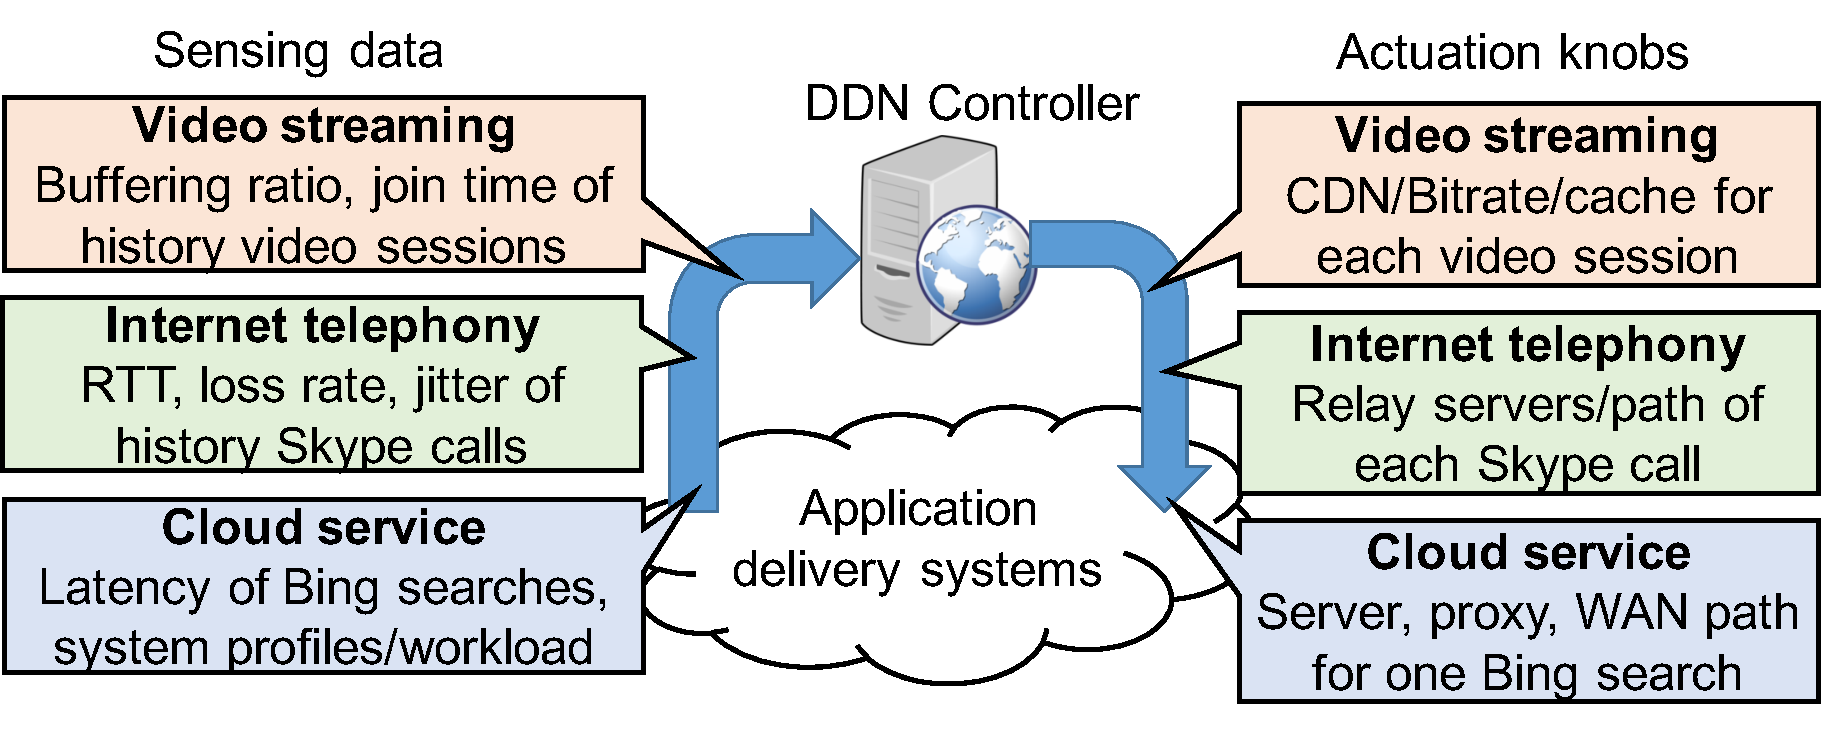
\includegraphics[width=0.8\textwidth]{figures/early-examples.pdf}
%%\vspace{-0.2cm}
%\caption{Examples of \ddn.}
%\label{fig:early-examples}
%\end{figure}



%\begin{figure}[t!]
%\centering
%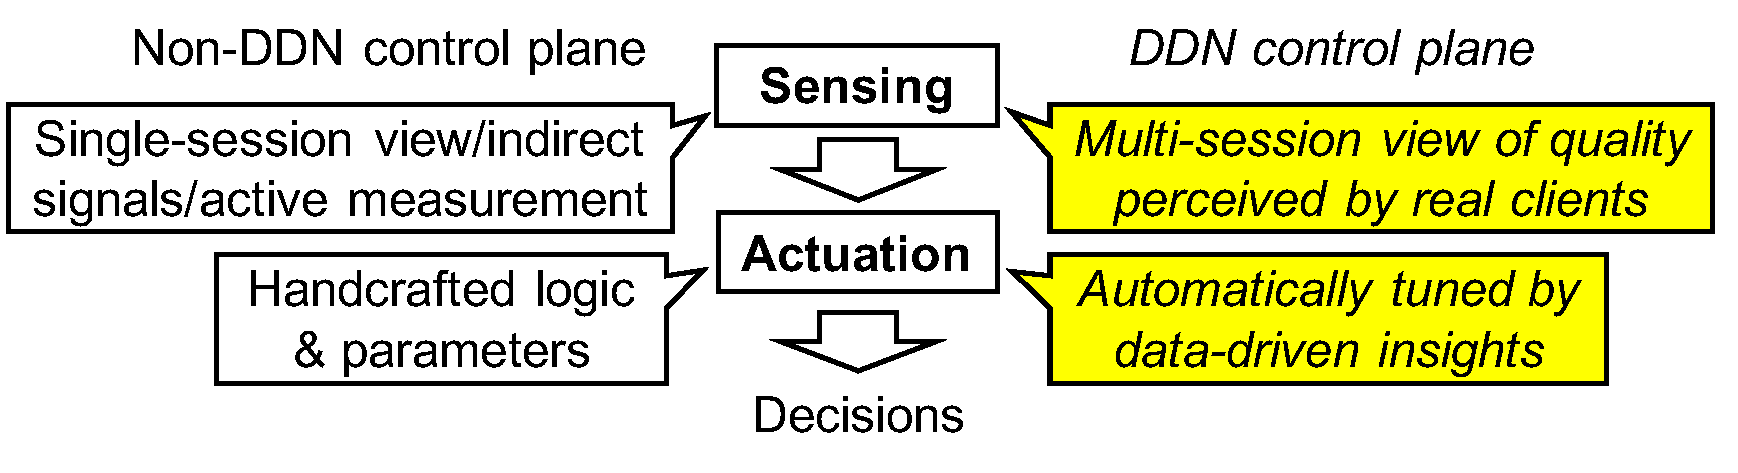
\includegraphics[width=0.8\textwidth]{figures/sensing-actuation.pdf}
%%\vspace{-0.7cm}
%\caption{\ddn control plane is fundamentally different to non-\ddn ones on both sensing and actuation.}
%\label{fig:sensing-actuation}
%\end{figure}


\section{Challenges}
\label{sec:overview:challenges}

While \ddn is promising,
it poses technical challenges on both 
algorithmic and architectural fronts, which have to be 
addressed before we can unleash its full potential.
%This section describes two fundamental challenges 
%of \ddn and how they manifest themselves in various
%applications.

\subsection{Need for Expressive Models}
\label{subsec:overview:challenge1}

Algorithmically, the objective of \ddn is to identify 
the best decision for each application sessions;
essentially, a mapping between the feature space
of application sessions and the decision space.
This is, however, by no means trivial even for 
standard machine learning techniques,
because the mapping is in a 
{\em high-dimensional} space.
Therefore, the key algorithmic challenge is 
how to build an expressive model to reduce
the dimensionality of both session-level 
feature space and decision space.
To make it more concrete, we discuss two
manifestations of the challenge of an expressive
model.

\begin{itemize}

\item {\em Complex QoE-determining factors:} 
The first example shows that the relation between
session-level features and video QoE is complex
both spatially and temporally.
Prior work has shown that there is a substantial room for 
improving video QoE by dynamically selecting the 
optimal CDN and bitrate based on a real-time global 
view of network conditions.
The key to realizing this promise is a prediction 
model that can accurately predict the quality of any 
video session based on QoE of similar sessions,
if it were to use any CDN and bitrate.
One challenge to practically build such prediction 
model is that video QoE has complex relationship to 
session-level features.
In particular, we observe a combinational effect
where QoE is affect by a specific combination 
of feature values, but does not appear to be 
correlated with any individual feature.
We also observe that QoE of different sessions 
may be affected with different feature combinations.
In addition to these spatial patterns, these 
QoE-determining factors, as well as QoE itself may
over time on timescales of several minutes.
Therefore a prediction model must be expressive
enough to capture all these spatial and temporal
complexities.

\item {\em Large decision spaces:}
The second example shows the problem of 
large decision spaces in Internet telephony.
Prior work has shown that there is much room 
for improving Skype quality by routing each 
call through the optimal relay clusters in 
the cloud.
%challenge
However, identifying a close-to-optimal relay 
in practice is very challenging, due to the sheer 
number of possible relay paths (in hundreds) and 
their dynamic performance (which could change 
on timescales of minutes). 
In addition, the number of calls different AS pairs
follows a highly skewed distribution, so that
in many AS pairs, the number of calls in each 
hour is even less than the number of possible 
relays.
Straightforward methods are not 
efficient to reduce the decision space.
For instance, focusing only on relays with 
the lowest geo-distance to end users
does not necessarily guarantee low latency, 
low packet loss rate which have been shown
to have weak, if any, correlation with the geo-distance.
Moreover, the best choice of relays depends 
on locations of both caller and callee.
All these evidences suggest a strong need
to reduce the size of the mapping between
the client space and the decision space in 
the context of today's VoIP architecture.

\end{itemize}



%\begin{itemize}
%\item From data to insights requires expressive models
%\item Example 1: predictive model
%\item Example 2: reducing decision space
%\end{itemize}

\subsection{Need for Scalable Platforms}
\label{subsec:overview:challenge2}

The system design of \ddn should meet the following requirements:
the \ddn controller has to make control decisions 
in near real time based on fresh data from many
other geo-distributed clients, and serve the decisions 
to clients within low response time.
The key architectural challenge, therefore,
is how to strike a balance between three seemingly
conflicting objectives: 
(1) {\em data freshness}, 
(2) {\em responsiveness to geo-distributed clients},
and (3) {\em global view}.
To make it more concrete, we again discuss two 
manifestations of the challenge of a scalable platform.

\begin{itemize}
\item {\em Geo-distributed analytics with global view:} 
The first example shows why it is challenging to 
make decision with a fresh, global view of QoE of 
many geo-distributed clients.
Although in theory, the \ddn controller can be 
integrated to the existing logically centralized control 
platforms deployed by many application providers,
there is a practical challenge: these control platforms 
are built up to serve two functions--
real-time per-session monitoring and 
offline analytics, neither of which requires a fresh 
and global data collected all clients, so it would be 
impractical to assume the decision-making algorithm 
can run in a cluster which has a fresh, global view 
of measurement data from all clients. 
Besides, it is costly to gather all data into one cluster,
because it requires to change the existing 
data gathering procedure and to significantly increase 
the communication overhead.
Therefore, one challenge is to 
perform geo-distributed analytics by striking a 
balance between global view and data freshness.

\item {\em Near real-time predictive analytics:}
Even if we can gather real-time data to the same data 
center, it is still very challenging to run real-time 
analytics to predict the optimal decision in near 
real time, e.g., on a timescale of tens of seconds.
As mentioned in 
Section~\ref{subsec:overview:challenge1},
to update quality prediction, we need a large amount 
of data to build a high-dimensional model between 
session-level feature space and QoE.
Our evaluation based on standard large-scale
analytics platforms has shown that it would take
tens of minutes, a magnitude longer than needed,
to update the model, given the sheer volume of
measurement data.

\end{itemize}

%\begin{itemize}
%\item From insights to real-time control requires scalable platform
%\item Example 1: Enabling complex real-time analytics
%\item Example 2: High responsiveness
%\end{itemize}


\section{Persistent Structures in QoE-Determining Factors}
\label{sec:overview:unifying}

%\jc{add a formal definition and illustrative figures of persistent structures}

Our solutions to address these challenges integrate 
standard ML algorithms and 
systems with a key domain specific insight that Internet
%Before we show how to address these challenges, 
%it would be helpful to  first understand the key domain-specific insight that
%inspires our solution.
%One unifying theme behind these seemingly 
%independent ideas is to integrate 
%standard machine learning algorithms and 
%systems with the domain-specific insight that Internet 
applications have {\em persistent structures
(e.g., performance bottlenecks) that help identify 
network sessions with 
similar QoE-determining factors, and that such 
structure tends to be persistent on timescales of 
at least tens of minutes}.
In Chapter~\ref{ch:measurement}, we will show evidence of these persistent
structures through an empirical structural analysis on  QoE
problems based on real datasets.
For now, we will give an overview of persistent structures 
and how intuitively they help address \ddn's challenges.

\mypara{Formal definition}
To formally describe the insight of persistent structures, 
let us formally describe \ddn as follows. In essence, \ddn is as 
a decision-making function
$F:2^\mathbb{S}\times2^\mathbb{D}\times\mathbb{S}\times\mathbb{R}
\mapsto\mathbb{D}$ which takes as input a set of historical 
sessions $S\in2^\mathbb{S}$ whose 
QoE is already measured, a set of available decisions 
$D\in2^\mathbb{D}$, a new session $s\in\mathbb{S}$, and $s$'s timestamp
$t\in\mathbb{R}$,
and outputs a decision $d\in\mathbb{D}$ for session $s$.
Then we formally define a {\em structure} as
a function 
$P:2^\mathbb{S}\times2^\mathbb{D}\times\mathbb{S}\times\mathbb{R}
\mapsto2^\mathbb{S}\times2^\mathbb{D}$,
which takes as input a pair of a set of historical 
sessions $S\in2^\mathbb{S}$ and a set of decisions $D\in2^\mathbb{D}$,
and a session $s\in\mathbb{S}$, and the timestamp
$t\in\mathbb{R}$, and outputs a pair of  subset of history sessions
$S'\subset{S}$ and a  subset of available decisions $D'\subset{D}$.



\mypara{Key properties}
Persistent structures have two key properties:

\begin{itemize}

\item {\em Criticality:} Spatially, these structures identify (often small) 
subsets of history
sessions and decisions which are more critical than others history sessions 
or decisions in determining QoE; i.e.,
$F(S,D,s,t)=F(S',D',s,t)$, where $(S',D')=P(S,D,s,t)$. This essentially
means the \ddn control logic can make almost the same decisions by
focusing on a subspace of relevant history sessions and decisions.

\item {\em Persistence:} Temporally, these structures tend to persist
on timescales of tens of minutes. This means in a time window $\Delta$ 
of  tens of minutes, the function $P$ is likely 
to find the same relevant history sessions and decisions,
i.e., $P(S,D,s,t)=P(S,D,s,t+\Delta)$.

\end{itemize}


\mypara{An example}
These persistent structures of QoE-determining factors can 
manifest themselves in many forms.
For instance, if the QoE of a video session depends on
the server load (i.e., some decision-specific properties)
and client-side ASN (i.e., some session-level features), and such
dependency lasts for tens of minutes,
then it would be possible to identify the best decision for
the session by looking
at history sessions having in the same AS 
(instead of all history sessions), and only consider server with 
low load (instead of all possible decisions).

\mypara{Intuition behind persistent structures}
The intuitive explanation of these persistent structures 
is that in networked systems and application delivery  systems, performance
bottlenecks are often persistent, and the persistent structures
can be viewed as ``manifestations'' of these bottlenecks in the space of 
session-level features and decision-specific properties--a session's QoE
only depend on history sessions and decisions 
experiencing the same bottleneck.
Such persistent bottlenecks can be found in many prior studies in the context
video streaming~\cite{cfa}, 
web service~\cite{footprint}, end-to-end
network performance~\cite{zhang2001constancy}.
They can also be viewed as a generalization of the persistent 
network congestions, which can be mathematically explained based on queueing theory
(Chapter 6 of \cite{keshav2012mathematical}).

% For instance, video
%sessions with similar QoE from the same CDN/server tend to match on 
%client IP prefix~\cite{cfa,cs2p}. 
%Similarly, VoIP calls between the same ASes are likely to share the best
%relays~\cite{via},  and clients from  same /24 IP prefix will have
%similar web load time from the same edge proxy~\cite{footprint}.

%which takes as input a given set of historical 
%sessions $S\in2^\mathbb{S}$ and a new session $s\in\mathbb{S}$,
%and outputs a subset of history sessions $S'\subset{S}$; 
%and $L:2^\mathbb{D}\times\mathbb{S}\mapsto2^\mathbb{D}$, 
%which takes as input a given set of available decisions
%$D\in2^\mathbb{D}$ and a new session $s\in\mathbb{S}$,
%and outputs a subset of these decisions $D'\subset{D}$.


%For instance, the persistent critical features 
%(Section~\ref{subsec:overview:cfa}) can be
%viewed a kind of persistent structure which
%groups video sessions that match values on
%their critical features.
%The fact that there is a stable subset of 
%promising relay choices for each AS pair 
%(Section~\ref{subsec:overview:guided}) 
%can be viewed as another example of 
%persistent structure, where the structure
%is the subspace of the large decision space.

\mypara{Why they are helpful}
Persistent structures are the key
enabler for our design of expressive models and scalable
systems for \ddn.
\begin{itemize}

\item First, the locality property of these domain-specific structures 
means they are in relatively low dimensional space.
%(e.g., in Section~\ref{subsec:overview:cfa}, 
%critical features are a small subset of all
%session-level features). 
Therefore, we can build models that focus on these 
domain-specific structures, so that 
they are expressive enough to capture the complex relations 
between session-level features
and decisions with limited available data, 
while avoiding using unnecessarily high-dimensional models.
This idea in spirit is similar how ``locality''
is used in many machine learning techniques 
to tackle curse of dimensionality~\cite{ml101}.

\item Second, in the context network applications,
these structures often correlate with network locality (e.g., clients 
in the same IP prefix). Therefore, they enable an effective spatial 
decomposition of the global 
data-driven process into smaller-scale 
subprocesses, each controlling a subset of 
sessions who share network locality.
% (i.e., can be mapped
%to the same subspace of relevant history sessions and decisions.
%(as in group-based exploration-exploitation of 
%Section~\ref{subsec:overview:group})
%or a subset of decisions (as in guided 
%exploration of 
%Section~\ref{subsec:overview:guided}).

\item Third, since these structures tend to
persist on longer timescales than QoE itself 
does, we can learn these structures from
more history data 
%(as in critical feature analysis of
%Section~\ref{subsec:overview:cfa} 
%and guided exploration of 
%Section~\ref{subsec:overview:guided}) 
with an
offline process separate from real-time 
decision making.
%(as in group-based 
%exploration-exploitation of
%Section~\ref{subsec:overview:group}).

\end{itemize}


\section{Key Ideas}
\label{sec:overview:solutions}

This section briefly describes three key ideas inspired by 
persistent structures
to address the aforementioned challenges. 
Figure~\ref{fig:overview-roadmap} summarizes the 
the mapping between the challenges and the ideas.
%We conclude the section by discussing a unifying
%insight underlying these solutions.

%of 
%{\em persistent structures--there exist some structure
%(e.g., performance bottlenecks) that identifies 
%network sessions with 
%similar QoE-determining factors, and that such 
%structure tends to be persistent on timescales of 
%tens of minutes}.
%The term ``structure'' is broadly defined, and will 
%have specific meanings when we discuss it in 
%context.
%Next, we will briefly describe how the persistent
%structures 

\begin{figure}[t!]
\centering
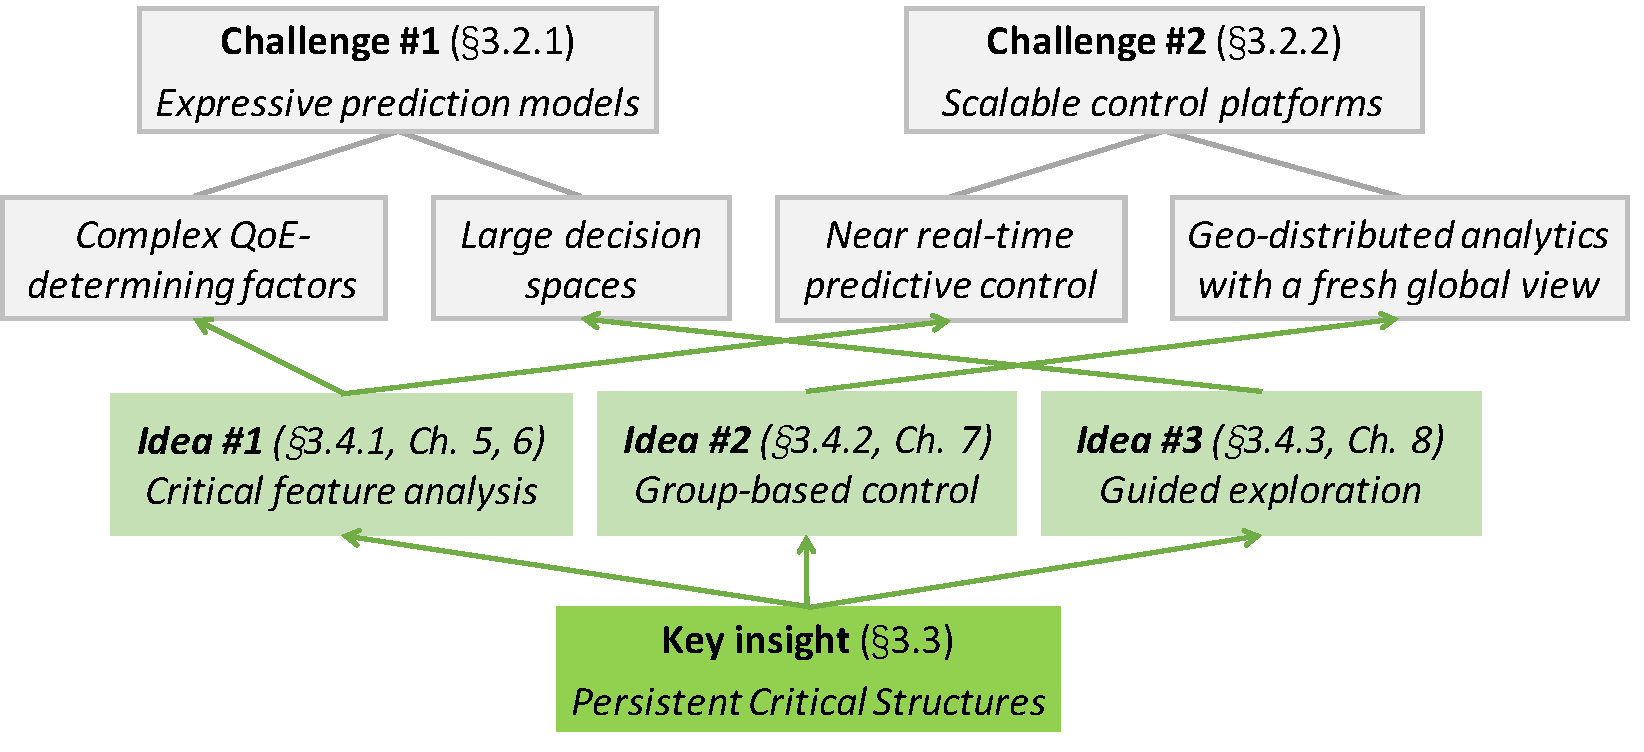
\includegraphics[width=0.95\textwidth]{figures/overview-roadmap.pdf}
%\vspace{-0.3cm}
\caption{Roadmap of the dissertation.
The figure shows that the unifying insight inspires 
our three key ideas to address four manifestations of
\ddn's key algorithmic and architectural challenge.}
\label{fig:overview-roadmap}
\end{figure}

\subsection{Critical Features Analysis}
\label{subsec:overview:cfa}

As we have seen, video QoE can be improved by
a prediction system that accurately predicts the QoE 
of a video session if it uses a certain CDN and bitrate.
The challenge is that this prediction system must be 
(a) expressive enough to capture complex relations 
between video quality and observed session features, 
and (b) capable of updating quality predictions in near 
real time.
We used several off-the-shelf machine learning 
techniques, such as random forests and SVM, but 
found they did not produce expected QoE improvements, 
because the long-term historical data is too coarse grained 
for these algorithms to capture the dynamics of video 
quality, while the short-term historical data is not sufficient 
for the algorithms to learn complex relations between 
video quality and observed session features.

Our solution leverages an instantiation of persistent structures
in video streaming, called 
{\em persistent critical features: each video session has 
a small set of critical features that ultimately determines 
its video quality, and these critical features change much 
more slowly than video quality}. 
Let us consider a concrete example of such persistent 
critical features from~\cite{cfa}.
In a real-world incident, video sessions of Comcast
users in Baltimore who watched videos from Level3
CDN experienced high failure rate (VSF) for several
hours. The reason turned out
to be the overloaded local cluster serving Comcast
users in that area,
which can be characterized by three critical features: 
CDN (``Level3''), ASN (``Comcast'') and City (``Baltimore''),
and the correlation between the combination of these
feature values and high VSF persist for the whole
duration of this incident, even though the QoE
has fluctuated a lot during this period.

The insight of persistent critical features has inspired
a prediction model that captures complex QoE-determining 
factors and is amenable to scalable implementation.
Given a video session under prediction, the model 
identifies many similar sessions from a short-term 
history by matching only on its critical features,
thus capturing complex QoE determining factors
while avoiding curse of dimensionality.
The persistence of these critical features also naturally
enables decoupled implementation: 
we can learn these critical features from long-term historical 
data and update the models by short-term historical data 
in near real time to capturing quality fluctuation.


%%\paragraph{CFA: Improving QoE via Expressive Prediction Models.}
%%problem
%Delivering high QoE is crucial to the success of today's subscription-/ad-based business models for Internet video.
%There is substantial room for improving video QoE by dynamically selecting the optimal CDN (Content Delivery Network) and bitrate based on a real-time global view of network conditions~\cite{sigcomm-case,conext-shedding}.
%The key to realizing this promise is a {\em prediction oracle} that can accurately predict the quality of a video client if it uses a certain CDN and bitrate.
%%challenge
%The challenge is that this prediction system must be (a) expressive enough to capture complex relations between video quality and observed session features, and (b) capable of updating quality predictions in near real time.
%We used several off-the-shelf machine learning techniques, such as random forests and SVM, but found they did not produce expected QoE improvements, because the long-term historical data is too coarse grained for these algorithms to capture the dynamics of video quality, while the short-term historical data is not sufficient for the algorithms to learn complex relations between video quality and observed session features.
%%these algorithms fail to capture the quality variability when trained with long-term history data, and they fail to identify the complex prediction models when trained with short-term history data.
%%Unfortunately, several seemingly natural solutions (e.g., simple machine learning approaches and network models) fail on one or both fronts.
%%insight
%My solution, CFA~\cite{cfa}, leverages the domain-specific insight of {\em persistent critical features}; each video session has a small set of critical features that ultimately determines its video quality, and these critical features change much more slowly than video quality~\cite{conext-shedding}. 
%%I present the design and implementation of CFA~\cite{cfa} to address these challenges. 
%%CFA is driven by the domain-specific insight of {\em persistent critical features}, that each video session has a subset of critical features that ultimately determines its video quality, and these critical features tend to be persistent on timescales of tens of minutes~\cite{conext-shedding}. 
%%solution
%This insight enables us to learn complex prediction models from long-term historical data (thus expressing complex relations between video quality and session features), and update the models by short-term historical data in near real time (thus capturing quality fluctuation as well).
%%Therefore, CFA can predict video quality more accurately than many machine learning algorithms, though CFA may not be as good in other prediction tasks.
%%result
%A real-world pilot deployment shows that CFA leads to non-trivial improvements in video quality, e.g., 32\% less buffering time than industry-standard algorithms.
%Our conversation with domain experts confirmed that these improvements are significant for content providers and can potentially translate into substantial benefits in revenues.
%An end-to-end implementation of CFA has been deployed and used by Conviva, a company that offers video quality optimization services to many premium content providers. 
%
%The insight of persistent critical features turns out to be more general; e.g., I have also applied the same insight to accurate prediction of TCP throughput~\cite{cs2p}, which leads to 11\% higher video bitrate than state-of-the-art adaptive bitrate players (e.g., Netflix players) with no extra buffering.


\subsection{Group-Based Control}
\label{subsec:overview:group}

While the predictive decision-making algorithm 
described above shows promising QoE improvement, 
it faces has two fundamental limitations.
(a) Casting the data-driven QoE optimization as a
prediction problem suffers from the many known 
biases such as incomplete visibility.
%A natural solution is to re-cast the problem
%as a real-time exploration and exploitation process,
%which however, is not trivial due to the fact that 
%measurement data of one client is useful only
%to the clients sharing the same QoE-determining
%factors.
(b) The prediction algorithm is not a geo-distributed one, 
so it requires a fresh and global view be maintained in
one cluster. Having a fresh and global view 
physically in the same cluster is, however, impractical 
because in many control platforms, measurement 
data are first collected in several geo-distributed frontend 
clusters each having a partial view of nearby clients,
and then periodically archived in a backend cluster
to form a global though slightly staled view.
A baseline approach is to run control logic in a 
single backend cluster with global data from frontend 
clusters, but this approach leads to non-trivial 
staleness of the global data and suboptimal decisions.


To overcome these limitations, we re-cast the 
data-driven QoE  optimization as a real-time 
exploration and exploitation process, and build 
a practical system to run it among all clients at 
scale. 
Our key insight is inspired by the criticality of persistent
structures -- {\em the clients that exhibit similar 
QoE behavior will have similar network-level 
features (e.g., same IP prefix), and thus their 
fresh data will likely be collected by the same 
frontend cluster.}
We see manifestations of this insight in many 
settings.
% When clients share certain location or IP prefix-related
%features, they are more likely to have the similar video QoE~\cite{cfa} and
%similar TCP throughput~\cite{cs2p,spand} at the same point of time. 
For instance, video sessions with similar QoE 
from the same CDN/server tend to match on 
client IP prefix~\cite{cfa,cs2p}. 
Similarly, VoIP calls between the same ASes 
are likely to share the best
relays~\cite{via},  and clients from  same /24 
IP prefix will have
similar web load time from the same edge 
proxy~\cite{footprint}.

This insight inspires the notion of {\em group-based 
control}, which enables the real-time global 
exploration-exploitation process by decomposing 
the process into subprocesses, each controlling 
a group of clients with similar context by
network locality and other key session-level features 
and running in the frontend cluster that has these 
clients' fresh data.
Since sessions within a group share network locality (e.g., 
in the same locations and IP prefixes), 
they are likely to be mapped to the same frontend cluster.
By running the per-group exploration-exploitation 
logic in this frontend cluster, we can update
decisions with fresh data from other sessions i
n the group received by this frontend cluster.


%%\mypara{\underline{\smash{Real-Time Exploration and Exploitation At Scale.}}}
%%\paragraph{Pytheas: Improving QoE via Exploration and Exploitation at Scale.}
%%\mypara{Real-Time Exploration and Exploitation at Scale:}
%%problem
%While formulating data-driven QoE optimization as a prediction 
%problem has shown promising QoE improvement (e.g., CFA), 
%it is necessarily incomplete, as 
%it suffers from many known biases such as incomplete visibility, 
%and cannot respond to sudden changes such as flash crowds.
%Drawing a parallel from machine learning (e.g., ad recommendation), I argued that data-driven QoE optimization should instead be cast as a {\em real-time exploration and exploitation} process. % rather than as a prediction problem. 
%Measurement collection (exploration) could be informed by decision making (exploitation) to explore the decisions with less data, thus addressing the shortcomings of the prediction-based formulation.
%This new formulation is complementary to CFA, since CFA's prediction model can be reused to capture similarities among clients.
%%challenge
%While many exploration-and-exploitation algorithms are available, enabling these algorithms in networking introduces an architectural challenge: we need a {\em scalable control platform} to update decisions with fresh global data from clients, despite data coming from a variety of geo-distributed front-end clusters, each with only a partial view of the clients.
%%The key challenge of real-time exploration and exploitation in networking is how to update decisions in real-time for millions of geo-distributed clients using their fresh measurement data.
%%insight
%A baseline approach is to run control logic in a single back-end cluster with global data from front-end clusters, but this approach leads to non-trivial staleness of the global data and suboptimal decisions.
%I take an alternative approach; the control logic is run by geo-distributed front-end clusters which have fresh data, rather than the back-end cluster.
%The intuition is that the clients that exhibit similar QoE behavior will have similar network-level features (e.g., same IP prefix), and thus their fresh data will likely be collected by the same front-end cluster.
%%While the challenge might be intractable in a general setting, it
%%I address the challenge by the insight that network application sessions sharing the same {\em network- and application-level features} intuitively exhibit similar QoE behavior across different possible decisions.
%%solution
%Inspired by this insight, {Pytheas}~\cite{pytheas} uses the concept of {\em group-based exploration and exploitation}, which 
%%The key idea is to decompose the global exploration and exploitation process of all clients into processes within groups of similar clients and run these per-group processes in geo-distributed front-end clusters which are close to clients and have their fresh data.
%%The key idea is to decompose the global exploration and exploitation process into subprocesses of similar clients, and run each subprocess by the front-end cluster that is close to its clients and has their fresh data.
%decomposes the global exploration and exploitation process into subprocesses, each controlling a group of similar clients and running in the front-end cluster that has these clients' fresh data.
%%with both client-closeness and data-freshness.
%%result
%Using an end-to-end implementation in CloudLab, I show that compared to a state-of-the-art prediction-based system, Pytheas improves the average video QoE by up to 31\% and the 90th percentile QoE by 78\%.
%Pytheas is an open source project that enables application providers to deploy the proposed architecture at scale within their existing infrastructure. 


\subsection{Guided Exploration}
\label{subsec:overview:guided}

To make data-driven QoE optimization practical in Internet telephony,
we have to address an additional challenge that it has a 
large decision space of relay choices, so there 
are usually not enough VoIP calls to reliably estimate 
the dynamic network performance between each 
AS pair.

The key insight to address this challenge is  another
illustration of persistent structure --
{\em the stability of promising relay choices: for each pair of 
caller AS and callee AS, there is a small and 
stable subset of relays that almost always 
contains the best relay}. 
This insight has two implications: 
(1) because this subset of relays is stable, 
it can be learned from history; and 
(2) because this subset has only a few relays 
(less than five), it can be explored efficiently 
even with limited data.
Inspired by this insight, we develop a relay selection 
system that achieved close-to-optimal quality 
using the concept of {\em guided exploration}. 
The idea is to learn a small set of promising relays 
for each AS pair based on long-term (e.g., daily) 
historical data, and explore these relays using most
calls in real time.

%%\mypara{\underline{\smash{Reducing Large Decision Space.}}} 
%%\paragraph{VIA: Improving QoE in the Face of Large Decision Spaces.} 
%%\mypara{Reducing Large Decision Space:}
%%problem
%In the first large-scale study on Internet telephony quality, I found that a substantial fraction of Skype calls suffer from poor network performance, and that there is much room for improving Skype quality by routing each call through the optimal relay clusters in Microsoft's cloud.
%%challenge
%However, identifying a close-to-optimal relay in practice is very challenging, due to the sheer number of possible relay paths (in hundreds) and their dynamic performance (which could change on timescales of minutes). 
%Neither prediction-based methods (e.g., CFA) nor those based on exploration and exploitation (e.g., Pytheas) suffice to handle such a large decision space.
%%insight
%The key insight to address this challenge is that, for each pair of caller ISP and callee ISP, there is a {\em small and stable subset} of relays that almost always contains the best relay. 
%This insight has two implications: (1) because this subset of relays is stable, it can be learned from history; and (2) because this subset has only a few relays (less than five), it can be explored efficiently even with limited data.
%%the large decision space can be narrowed down to a {\em small subset} of relays that almost always contains the best relay, and such pruning can be learned from the historical data, because this set of most promising relays tends to be {\em persistent}.
%%solution
%Inspired by these intuitions, I developed {VIA}~\cite{via}, a relay selection system that achieved close-to-optimal quality using the concept of {\em guided exploration}. The idea is to learn a small set of promising relays for each ISP pair based on long-term (e.g., daily) historical data, and explore these relays using most calls in real time.
%%result
%Trace-driven analysis and a small-scale deployment shows that VIA cuts the incidence of poor network conditions for calls by 45\% (and for some countries and ISPs by over 80\%) compared to today's Skype quality.
%VIA has been used in Microsoft internal deployment with real Skype users, and is in the process of being fully deployed. 
%VIA was also used by Microsoft to identify the countries and ISPs where Skype quality can benefit the most if relaying services are deployed.
%%VIA is also used to identify the countries and ISPs where Skype quality can benefit the most from Microsoft relaying services.


%\subsection{How Persistent Structures Are Used}
 


\section{Summary}

In this section, we have discussed the advantages
of \ddn over prior approaches. 
In particular, as an application-level endpoint 
approach, \ddn enjoys the advantage of direct 
access to user-perceived QoE, and at the same
time, compensates the limited insight to network 
conditions by consolidating real-time measurement
from many endpoints, thus achieving the best world
of both endpoint solutions and in-network solutions.

We have also presented an overview of our solutions
to address \ddn's technical challenges--the need for 
expressive models and scalable systems. 
In particular, there are the three key ideas underlying 
our solutions: 
(1) critical feature analysis to enable an expressive 
QoE prediction model, 
(2) group-based control to enable real-time 
exploration-exploitation process at scale, and
(3) guided exploration to handle the large 
decision spaces in Internet telephony.
Finally, we summarize the section by distilling 
a unifying insight from these 
ideas--\ddn can be made practical by integrating
machine learning with the insight that there are 
persistent domain-specific structures.







